\documentclass[landscape]{article}
\usepackage[polish]{babel}
%\usepackage{amsmath}
\usepackage{fancyhdr}
%\usepackage{dsfont}
\usepackage{graphicx}
\usepackage[utf8]{inputenc}
\usepackage[T1]{fontenc}
\usepackage{multirow}
%\usepackage{color}
%\usepackage[usenames,dvipsnames,svgnames,table]{xcolor}
%\usepackage{ulem}

\setlength{\parindent}{0pt}
\topmargin  -15mm
\oddsidemargin  -10mm
\textwidth  250mm
\textheight 167mm
\columnwidth 100mm
\frenchspacing
\sloppy
\setlength{\columnsep}{10mm}
\fancyhead{}
\rhead{\begin{tabular}{r} Creative Commons License:\\ Attribution Share Alike\end{tabular}\raisebox{-0.3\height}{
\includegraphics[height=0.7cm]{cc_cc_30}
\includegraphics[height=0.7cm]{cc_by_30}
\includegraphics[height=0.7cm]{cc_sa_30}}}
\chead{\LARGE\sc Info III: Lab \labnumber}
\lhead{\begin{tabular}{rl}Autor:&{\it\autorone}\\{\it\autortwo}&\end{tabular}}
\rfoot{\thepage}
\cfoot{}
\lfoot{\it Wydział Mechaniczny Energetyki i Lotnictwa, Politechnika Warszawska}
\twocolumn
\pagestyle{fancy}
\newcommand{\red}{\color{Red}}
\newcommand{\green}{\color{Green}}
\newcommand{\blue}{\color{Blue}}
\newcommand{\newtitle}{{\huge\begin{center}{\sc Informatyka III: Instrukcja \labnumber}\\{\it\mytitle}\end{center}}}

%%%%%%%%%%%%%%%%%%%%%%%%%%%%%%%%%%%%%%%%%%%%%%%%%%%

\newcommand{\autorone}{M. Dzikowski}
\newcommand{\autortwo}{}
\newcommand{\mytitle}{}
\newcommand{\labnumber}{1}

\begin{document}
\newtitle

\section{Podstawy pracy z systemem UNIX}

Większość współczesnych komputerów (i podobnych urządzeń, np tablety czy telefony) wyposażonych jest w złożone oprogramowanie które składa się na system operacyjny. Z całą pewnością korzystałeś z systemów firmy Microsoft czyli rodziny Windows. Mogłeś też zetknąć się z Android'em  (czyli odmianą UNIXa) od Google czy iOS od Apple. W większości przypadków system posiada tzw. interfejs graficzny czyli GUI. Większość z nich jest zasadniczo podobna i np. uruchomienie przeglądarki internetowej czy przeglądanie dysku nie jest dla nikogo wyzwaniem.

Jednak nie każdy komputer posiada GUI, dotyczy to głównie dużych komputerów używanych w poważnych obliczeniach numerycznych (np. wyznaczanie właściwości aerodynamicznych samochodu z użyciem Fluent'a). W takim przypadku nie ma możliwości skorzystania z klawiatury i myszki czy podejrzenia czegoś na ekranie, ponieważ komputer znajduje się w serwerowni, czasami w innym kraju. Aby korzystać z takiego zdalnego komputera musimy połączyć się z nim przy pomocy specjalnego programu, następnie wydajemy mu polecenia w trybie tekstowym.

Na potrzeby tego laboratorium każdy otrzymał kartkę z loginem i hasłem. Są one ważne do końca semestru i można przy ich pomocy zalogować się na nasz szkolny serwer również spoza kampusu.

Gdy korzystasz z Windows'ów najwygodniej do połączenia wykorzystać darmowy program PuTTy. Po uruchomieniu pokaże się okno jak na obrazku obok. Należy podać:
\begin{itemize}
\item {\tt Hostname }-- nazwa hosta, czyli {\tt info3.meil.pw.edu.pl}
\item {\tt Port}-- Numer portu z których chcemy się połączyć, czyli 22, oraz protokół {\tt SSH} z listy poniżej
\end{itemize}


%\begin{figure}[ht!]
%\centering
%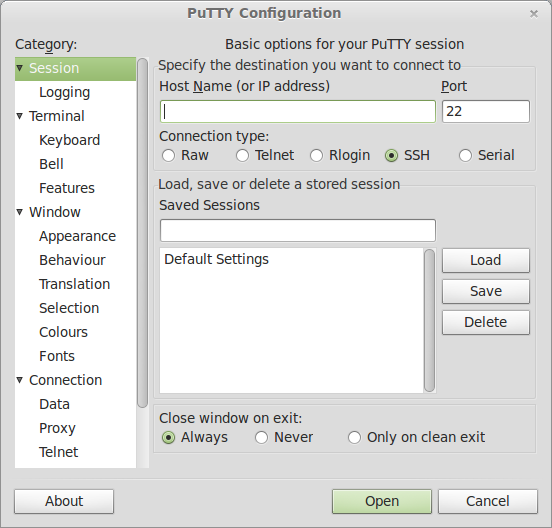
\includegraphics[width=60mm]{putty_004.png}
%\caption{Główne okno programu PuTTy}
%\label{overflow}
%\end{figure}

Następnie pojawi się czarne okno z zapytaniem o login i hasło. Po podaniu i poprawny zalogowaniu zobaczysz informacje o dacie, licencji, wersji systemu itp. kończące się:

\begin{verbatim}
Last login: Thu Feb 21 06:23:38 2013 from xx.xx.xx.xx
stud-00@info3:~$
\end{verbatim}

Zapis:
\begin{verbatim}
stud-00@info3:~$
\end{verbatim}
oznacza, że jako użytkownik {\tt stud-00} jesteśmy zalogowani na komputer {\tt info3}. Między znakami : i  \$ znajduje się aktualny katalog. W tym przypadku \~, czyli katalog domowy, inaczej {\tt /home/students/stud-00 }

\section{Ćwiczenia}
\subsection{Pierwsze starcie}

Wpisz do konsoli {\tt date} i wciśnij enter. Komputer wyświetli aktualną (jego zdaniem) datę. następnie ponownie wyświetli linijką kończącą się na \$, oznaczającą że czeka na polecenia. Używając strzałki do góry możesz przeglądać historię poleceń. Jeśli wpiszesz {\tt dat} i naciśniesz 2x klawisz tab, wyświetlona Ci zostanie lista poleceń zaczynających się na {\tt dat} lub jeśli jest tylko jedno, nazwa zostanie dokończona. Pamiętaj o tych 2 trikach, bo znacznie ułatwiają pracę w trybie tekstowym.

\subsection{Poruszanie się po katalogach}

Pracując w trybie tekstowym, zawsze pracujemy w jakimś katalogu, tzw. katalogu bieżącym. Jeśli uruchomimy jakiś program, np. proste programy czytające z pliku z Informatyki I, będą one czytały z plików w tym katalogu. Każdemu programowi którego będziesz używać a który potrzebuje nazwy pliku lub katalogu (np. do kopiowania) może ją przyjąć w kilku postaciach. Po pierwsze ścieżka  bezwzględna, zaczynająca się od znaku / np:
\begin{verbatim}
/home/students/stud-00
/usr/bin/bash
/etc
\end{verbatim}

Sprawdź, w jakim katalogu się znajdujesz, wpisz {\tt pwd} i wciśnij enter.

Aby zmienić katalog, wykorzystuje się polecenie {\tt cd}, np.
\begin{verbatim}
stud-00@info3:~$ cd /tmp
stud-00@info3:/tmp$ pwd
/tmp
\end{verbatim}

Teraz przejdź do katalogu {\tt /home} i sprawdź czy się udało, z użyciem polecenia {\tt pwd}

Dodatkowo, oprócz ścieżki bezwzględnej, można podać nazwę katalogu który nas interesuje na kilka innych sposobów.

\begin{itemize}
\item $\sim$  zawsze oznacza katalog domowy
\item {\tt ../} oznacza katalog nadrzędny
\item {\tt /} oznacza katalog główny, początek każdej ścieżki bezwzględnej
\item {\tt .} i {\tt ./} oznacza katalog bieżący, ten zwracany przez {\tt pwd}
\end{itemize}

Przejdź teraz z powrotem do katalogu domowego i sprawdź czy się udało. Następnie 2 razy przejdź katalog wyżej i sprawdź, czy katalog bieżący to {\tt /home}

\subsection{Tworzenie i usuwanie katalogów}

Do tworzenia katalogów służy polecenie {\tt mkdir} np.
\begin{verbatim}
stud-00@info3:~$mkdir nazwa_katalogu
\end{verbatim}

a do sprawdzenia zawartości aktualnego katalogu polecenie {\tt ls}. Stwórz teraz katalogi A,B,C i D, każdy wewnątrz poprzedniego. Będziesz musiał stworzyć katalog A, przejść do niego, stworzyć B itd.
Do usuwanie katalogów służy polecenie {\tt rmdir}. Usuń teraz stworzone katalogi.

UWAGA: nie można w ten sposób usunąć katalogu posiadającego zawartość

\section{Podstawowe operacja na plikach i katalogach}
Komenda {\tt echo } wypisuje na ekran ciąg znaków który podaje się jej jako argument. Sprawdź.
Aby stworzyć pierwszy plik wpisz (o znaczeniu {\tt >>} będzie na kolejnych zajęciach)
\begin{verbatim}
stud-00@info3:~$echo pierwszy plik >> plik.txt
\end{verbatim}

Aby wyświetlić zawartość pliku a ekranie używamy {\tt cat}

\begin{verbatim}
stud-00@info3:~$cat plik.txt
\end{verbatim}

\subsection{Kopiowanie i przenoszenie}

Do kopiowanie służy komenda {\tt cp CO GDZIE}. Stwórz teraz katalog i skopiuj do niego twój plik. Powinno to wyglądać tak:
\begin{verbatim}
stud-00@info3:~$cp plik.txt katalog
\end{verbatim}

Aby przenieść/zmienić nazwę pliku lub katalogu używamy {\tt mv CO GDZIE}. Przejdź do nowego katalogu i zmień nazwę pliku. Następnie usuń plik poleceniem {\tt rm}

\section{Pomoc}
Znakomita większość komend trybu tekstowego posiada porządną dokumentację dostępną od ręki.
\begin{verbatim}
stud-00@info3:~$man rm
stud-00@info3:~$rm --help
\end{verbatim}
W przypadku komendy {\tt man} dostajemy kompetentniejszą dokumentację. Przewija się strzałkami, aby zakończyć wciśnij Q.
Sprawdź instrukcje dla poleceń {\tt who}, {\tt whoami}, {\tt finger} i  {\tt date}. Sprawdź jak działają.

\section{Program Tar}
Program {\tt tar} służy do pakowania i rozpakowywania drzewa katalogów i plików w jeden plik. Niekoniecznie musi on być mniejszy niż oryginalne pliki. Dopiero użycie kompresji zmniejszy objętość. Najpierw przygotuj kilka plików do spakowania:
\begin{verbatim}
stud-00@info3:~$ mkdir a
stud-00@info3:~$ cd a
stud-00@info3:~/a$ mkdir b
stud-00@info3:~/a$ echo asdasd >> ./b/c
stud-00@info3:~/a$ cat ./b/c
asdasd
\end{verbatim}

Teraz spakuj a nastnie podejrzyj archiwum programem {\tt mc}

\begin{verbatim}
stud-00@info3:~/a$ tar -cf test.tar b
stud-00@info3:~/a$ ls
b  test.tar
stud-00@info3:~/a$ mc
\end{verbatim}

Sprawdź zawartość katalogu, usuń to co przed chwilą spakowałeś do archiwum, następnie rozpakuj.

\begin{verbatim}
stud-00@info3:~/a$ ls
b  test.tar.gz
stud-00@info3:~/a$ rm -rf b
stud-00@info3:~/a$ ls
stud-00@info3:~/a$ tar -xf test.tar
stud-00@info3:~/a$ ls
b  test.tar
\end{verbatim}

Sprawdź poleceniem {\tt ls -la} objętość archiwum, zapisz, następnie spakuj te same pliki z dodatkową flagą {\tt z} zmieniając rozszerzenie na {\tt tar.gz}. Sprawdź czy plik wynikowy jest mniejszy.


\section{Proste skrypty}
Najważniejszym aspektem pracy w trybie tekstowym jest możliwość tworzenie skryptów, czyli zapisanych w pliku kolejnych komend wykonywanych tak, jakbyśmy wpisywali je z klawiatury. Więcej o zaawansowanych skryptach dowiesz się na następnych laboratoriach, pierwszy napiszesz dzisiaj.

Prostym i dość wygodnym edytorem tekstu jest {\tt nano} lub {\tt vim}. Uruchom go komendą {\tt nano NAZWAPLIKU} i zapisz do niego pierwszy skrypt:
\begin{verbatim}
#!/bin/bash
echo 1
echo 2
\end{verbatim}

Natępnie trzeba zmienić uprawnienia, pozwolić na uruchomienie naszego skryptu: 
\begin{verbatim}
stud-00@info3:~$ chmod +x skrypt.sh
stud-00@info3:~$ ./skrypt
\end{verbatim}

\subsection{Zmienne}
Bash obsługuje zmienne, jak w C. Aby stworzyć zmienną:
\begin{verbatim}
zmienna=$( JAKISPROGRAM )
zmienna=$( echo 1 )
\end{verbatim}

Aby odczytać zmienną:
\begin{verbatim}
echo $zmienna
\end{verbatim}

\subsection{Pierwszy skrypt}

Przygotuj strukturę katalogów:

\begin{itemize}
 \item AA
  \begin{itemize}
   \item BB
    \begin{itemize}
     \item plik.txt
    \end{itemize}
   \item CC
    \begin{itemize}
     \item DD
     \item plik.txt
    \end{itemize}
  \end{itemize}
\end{itemize}

zawierając komendy w skrypcie, plik ma zawierać datę z użyciem {\tt date}.

Zmodyfikuj skrypt tak, aby nazwa każdego katalogu zaczynała się od wielkości ze zmiennej {\tt \$1 }, która jest pierwszym argumentem skryptu w linii komend.

\begin{itemize}
 \item \$1\_AA
  \begin{itemize}
   \item \$1\_BB
    \begin{itemize}
     \item ...
    \end{itemize}
  \end{itemize}
\end{itemize}


\subsection{Pętle}
Przygotuj skrypt:
\begin{verbatim}
for i in *.txt
do
 cp $i $1_$i
done
\end{verbatim}
i uruchom go w katalogu z plikiem {\tt .txt}, jak działa? Pamiętaj o argumencie skryptu!


Napisz skrypt który tworzy katalog {\tt \$1} i kopiuje do niego wszystkie pliki .txt dodając przedrostek {\tt \$2}. Co się stanie jak nie podasz argumentów do skryptu?


\section{GUI}

Zresetuj komputer, uruchom Ubuntu i zaloguj się na konto quest. Używając menu z lewej strony uruchom terminal.

Połącz się programem {\tt ssh LOGIN@HOST} z serwerem info3. Utwórz plik {\tt copyme}.

Zakończ połączenie {\tt Ctrl+D}. Użyj programu 

\begin{verbatim}
scp LOGIN@HOST:SCIEZKA_DO_PLIKU GDZIE_KOPIOWAĆ} 
\end{verbatim}

aby ściągnąć {\tt copyme} na dysk lokalny. Program {\tt scp} działa tak jak {\tt cp}, z tą różnicą, że cel lub źródło znajduje się na innym komputerze obsługującym połączenia ssh.

\section{*Coś na deser}

\subsection{Pre-rekwizyty}
Sprawdź do czego służy program {\tt write} z użyciem {\tt man}. Użyj go. następnie porównaj "wyjście" komend: 
\begin{verbatim}
who
who | awk '{print $1}'
who | awk '{print $2}'
\end{verbatim}

\subsection{Skrypt spamera}

Stwórz skrypt:
\begin{verbatim}
#!/bin/bash
for u in $( who | awk '{print $1}' )
do
   echo $u
done
\end{verbatim}

następnie zmodyfikuj go tak, aby "zaspamować" wszystkich zalogowanych.

Kolejnym krokiem będzie dodanie do skryptu pakowania uzyskanego drzewka, następnie usuwanie oryginału.


\end{document}


